\documentclass[]{thesis-ekf}
\usepackage[T1]{fontenc}
\PassOptionsToPackage{defaults=hu-min}{magyar.ldf}
\usepackage[magyar]{babel}
\usepackage{mathtools,amssymb,amsthm,pdfpages,listingsutf8,hyperref}
\footnotestyle{rule=fourth}

\newtheorem{tetel}{Tétel}[chapter]
\theoremstyle{definition}
\newtheorem{definicio}[tetel]{Definíció}
\theoremstyle{remark}
\newtheorem{megjegyzes}[tetel]{Megjegyzés}

\begin{document}
	\institute{Matematikai és Informatikai Intézet}
	\title{Adatbázis alapú web alkalmazás fejlesztése}
	\author{Verebélyi Valentin\\Programtervező Informatikus BSc}
	\supervisor{Dr.~Tajti Tibor Gábor\\Egyetemi Docens}
	\city{Eger}
	\date{2024}
	\maketitle
	\tableofcontents
	
	\chapter*{Bevezetés}
	\addcontentsline{toc}{chapter}{Bevezetés}

	
	\chapter{Fejlesztés}
	\section{Fejlesztésről}
	\section{A fejlesztéshez alkalmazott eszközök és technológiák}
	\subsection{Laravel}
		A Laravel egy nyílt forráskódú, PHP webkeretrendszer, ami MVC tervezési mintán alapszik. Az MVC a Model-View-Controller rövidítése.
		\begin{enumerate}
			\item Model (Modell): ez az adatokat kezelő réteg, az adatok tárolásáért és visszaolvasásáért felelős.
			\item View (Nézet): ez a réteg felhasználói felületek megjelenítéséért illetékes. 
			\item Controller (Vezérlő): a felhasználói műveletek megfelelő kezeléséért ez a réteg a felelős.
		\end{enumerate}
		Mivel három részre van bontva, ezért van ennek a tervezési mintának néhány előnye is. Ilyen például ha lecseréljük az egyik réteget, akkor a többihez nem kell már hozzányúlni, amivel pénzt és időt is lehet spórolni. Előnye még az is, hogy egy modellnek lehet több nézetes is.
		\cite[102-103.~oldal]{Kusper}
		
	\subsection{PHP}
	\subsection{MySQL}
	\subsection{PhpMyAdmin}
	\subsection{XAMMP}
	\subsection{Visual Studio Code}
	\subsection{GitHub}
	\subsection{GitHub Desktop}
	
	
	\chapter{Tervezés}
	\section{Tervezésről}
	\section{A tervezéshez alkalmazott eszközök és technológiák}
	\subsection{PlantUML}
	\subsection{Dbdiagramm}
	
	\chapter{Tesztelés}
	\section{Tesztelésről}
	\section{A teszteléshez alkalmazott eszközök és technológiák}
	\subsection{Cypress}
	
	\chapter{Felhasználói dokumentáció}

	
	
	\chapter*{Összegzés}
	\addcontentsline{toc}{chapter}{Összegzés}
	
	\begin{thebibliography}{2}
		\addcontentsline{toc}{chapter}{\bibname}
		\bibitem{Kusper}
		\textsc{Kusper Gábor}: \emph{Programozási technológiák}, Eger, 2015.
	\end{thebibliography}
	
	% Aláírt, szkennelt nyilatkozat beillesztése a szakdolgozat végére
	%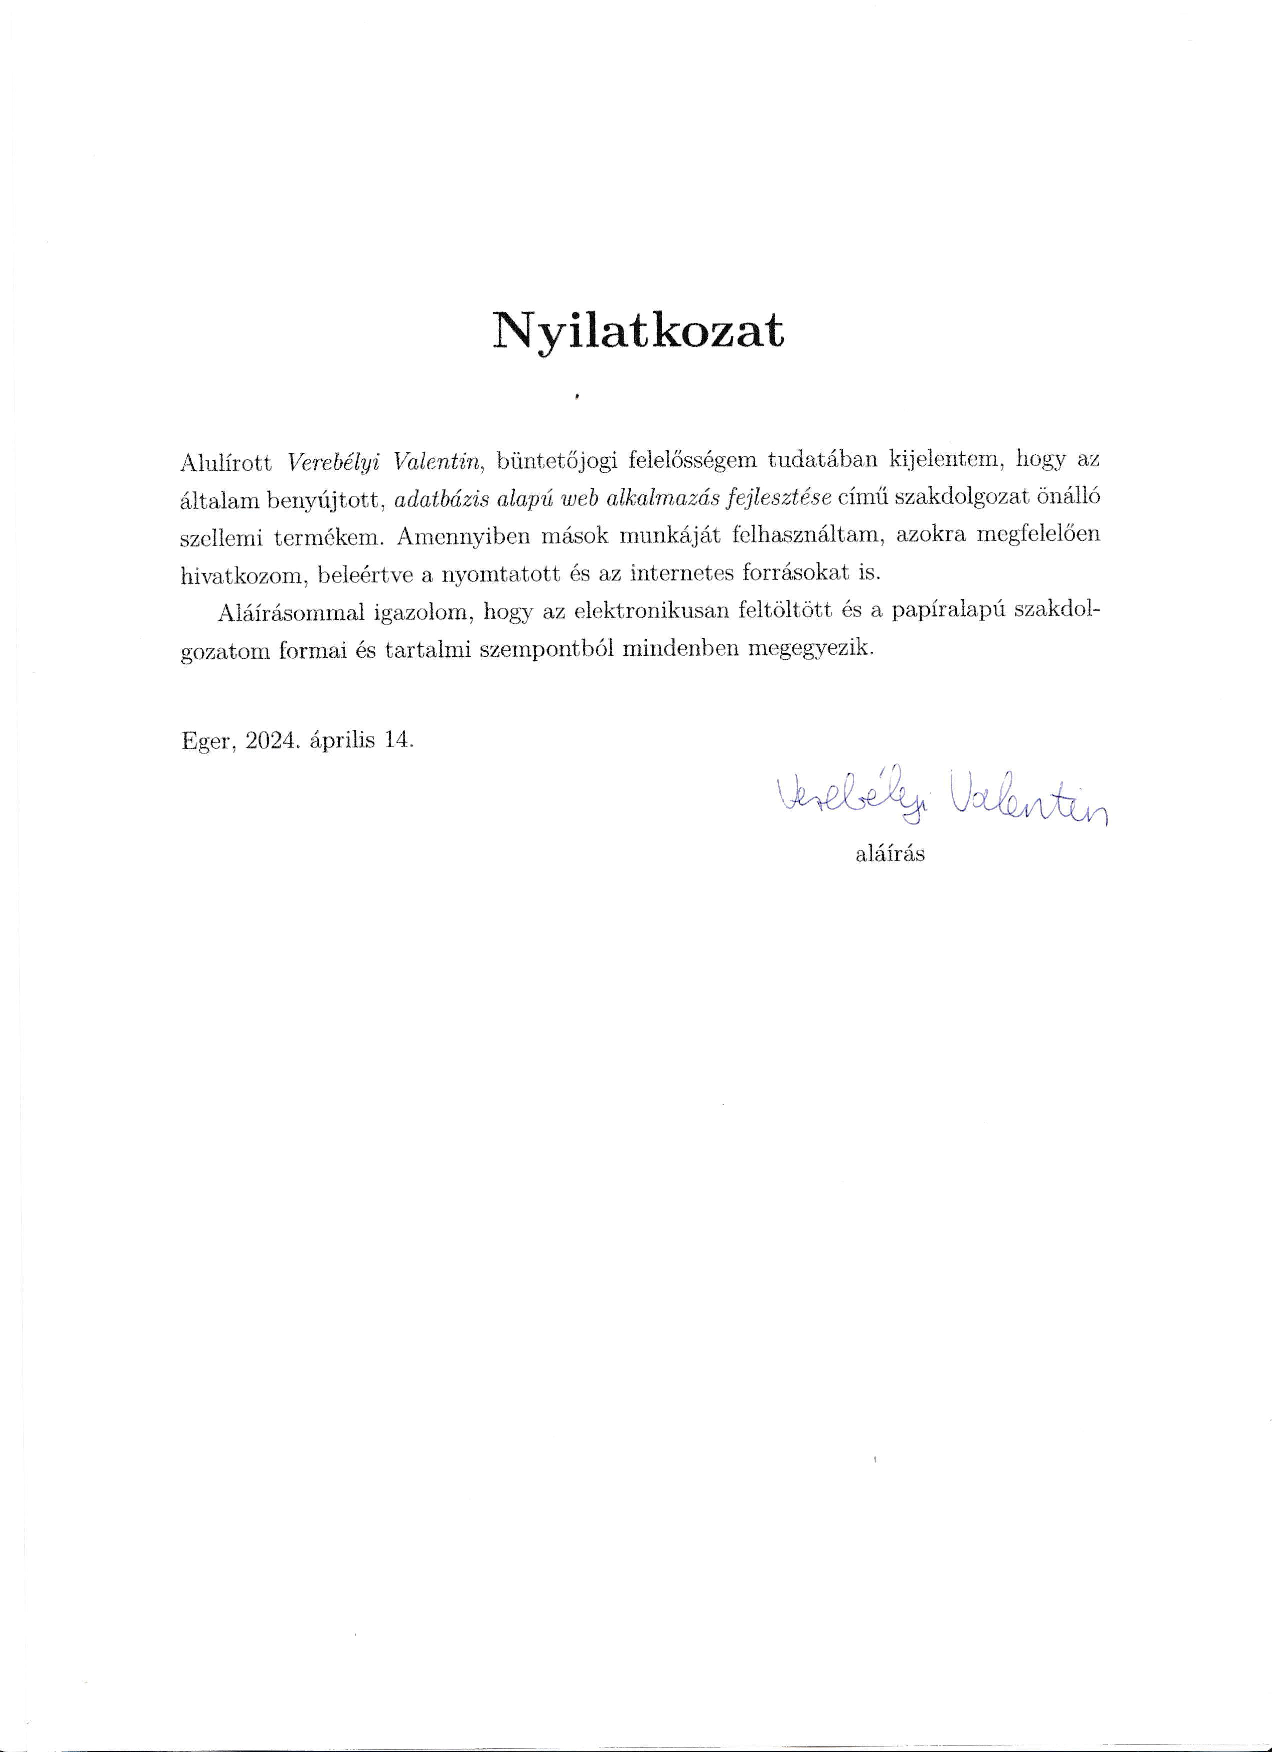
\includepdf{nyilatkozat.pdf}
\end{document}